\documentclass{article}

%% Bart Snapp

\usepackage{imfellEnglish}
\usepackage[T1]{fontenc}
\usepackage{graphicx}
\usepackage{tikz}


\usepackage[landscape,margin=1cm]{geometry}

%% from https://tex.stackexchange.com/questions/371906/how-to-draw-a-caesar-cipher-diagram-with-tikz

\usetikzlibrary{decorations.text,arrows.meta,calc}

\tikzset{curved text/.style={decorate,
        decoration={text effects along path,
            text={#1}, text align=center,
            text effects/.cd, text along path}}}

\begin{document}
\begin{center}
    \resizebox{!}{.9\textheight}{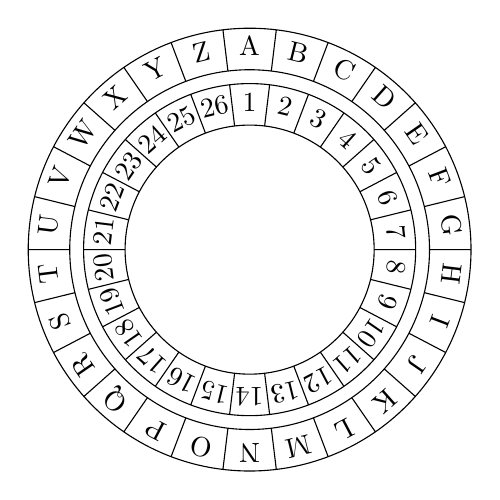
\begin{tikzpicture}[x=1em,y=1em]
%   set up
    \pgfmathsetmacro\angdiv{360/26}
    \pgfmathtruncatemacro\caeser{0} % Input Caeser shift here! (positive for clockwise)
    \coordinate (n-0) at (90+\angdiv/2:7) {};
    \coordinate (m-0) at (90-\caeser*\angdiv+\angdiv/2:5) {};
%   draw Caeser diagram 
    \draw circle [radius=8] circle [radius=6.5] circle [radius=6]  circle [radius=4.5]
        \foreach \i in {0,...,25}{%
            ($({90-(\i-1/2)*\angdiv}:8)$) -- ($(({90-(\i-1/2)*\angdiv}:6.5)$)
            ($({90-(\i-1/2)*\angdiv}:4.5)$) -- ($(({90-(\i-1/2)*\angdiv}:6)$)
        };
    \foreach [count=\a from 0] \text in {A,B,...,Z}{
        \pgfmathtruncatemacro\b{\a+1}%
        \path [curved text=\text] (n-\a) arc [start angle=90-(\a-1/2)*\angdiv, delta angle=-\angdiv, radius=7] node (n-\b) {};
        %\path [curved text=\text] (m-\a) arc [start angle=90-(\a+\caeser-1/2)*\angdiv, delta angle=-\angdiv, radius=5] node (m-\b) {}; % Inner circle
    }
    \foreach [count=\a from 0] \text in {1,2,...,26}{
        \pgfmathtruncatemacro\b{\a+1}%
        %\path [curved text=\text] (n-\a) arc [start angle=90-(\a-1/2)*\angdiv, delta angle=-\angdiv, radius=7] node (n-\b) {};
        \path [curved text=\text] (m-\a) arc [start angle=90-(\a+\caeser-1/2)*\angdiv, delta angle=-\angdiv, radius=5] node (m-\b) {}; % Inner circle
    }
    \end{tikzpicture}}
    \end{center}
\end{document}
